%##noBuild
\newpage
\section{Dziennik}

\subsection{2018-12-11}
Usiłujemy doprowadzić do działania otwarcie socketu dla serwera HTTPs i połączenie do niego.
Logi wskazują, że uzyskanie adresu z DHCP udaje się. Jednak późniejsza próba komunikacji 
z urządzeniem śledzona w Wiresharku wskazuje, że płytka nie odpowiada nawet na zapytania ARP o 
jej adres.

Dopisując wiele komunikatów debuagu odkrywamy, że HardFault następują podczas 
wywołania 
\begin{verbatim}
sys_arch_mbox_fetch(&conn->acceptmbox, &accept\_ptr, 0);
\end{verbatim}
w api\_lib.c:netconn\_accept
 

\subsection{2019-01-03}
Tym razem zwiększenie stosu ze 128 na 1024 przydaje się do rozwiązania problemów z ładowaniem 
certfikatów i inicjalizacją RNG.

Udaje się dotrzeć do początkowych wiadomości handshake’u, ale jeszcze nie zakończyć go:

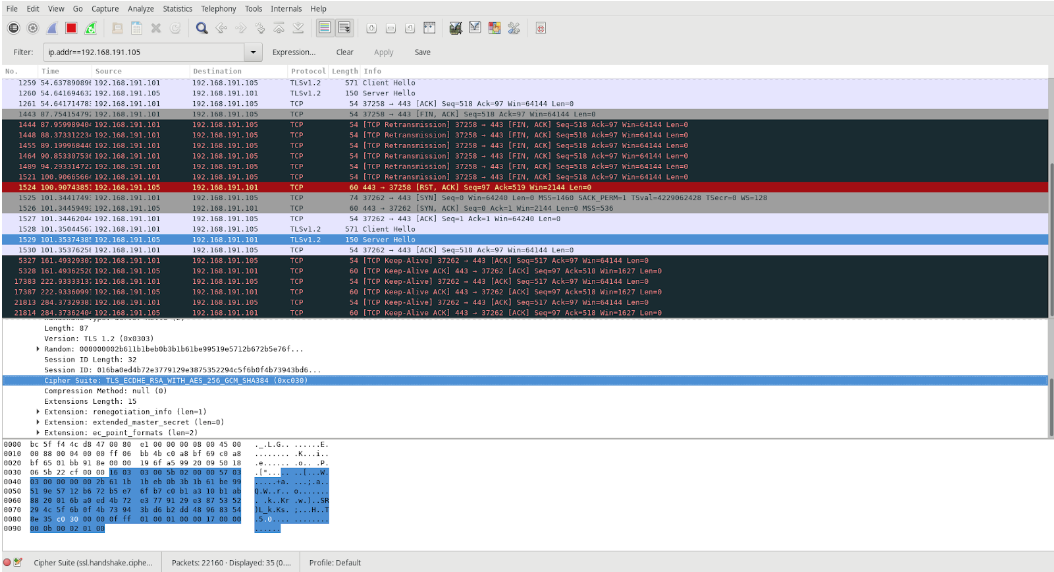
\includegraphics[width=\linewidth]{./images/1.png}


Okazuje się że problem leży raczej w curlu. Wówczas docieram jedynie do (dodawszy debugi w 
funkcji mbedtls\_ssl\_handshake):

\begin{verbatim}
mbedtls_ssl_handshake line 6560
mbedtls_ssl_handshake line 6563 state 0
mbedtls_ssl_handshake line 6567 ret 0 state 1
mbedtls_ssl_handshake line 6563 state 1
mbedtls_ssl_handshake line 6567 ret 0 state 2
mbedtls_ssl_handshake line 6563 state 2
mbedtls_ssl_handshake line 6567 ret 0 state 3
mbedtls_ssl_handshake line 6563 state 3
\end{verbatim}

Przy połączeniu z firefoksa (i zignorowaniu ostrzeżenia o nieznanym certyfikacie) - sukces:
\begin{verbatim}
mbedtls_ssl_handshake line 6560
mbedtls_ssl_handshake line 6563 state 0
mbedtls_ssl_handshake line 6567 ret 0 state 1
mbedtls_ssl_handshake line 6563 state 1
mbedtls_ssl_handshake line 6567 ret 0 state 2
mbedtls_ssl_handshake line 6563 state 2
mbedtls_ssl_handshake line 6567 ret 0 state 3
mbedtls_ssl_handshake line 6563 state 3
mbedtls_ssl_handshake line 6567 ret 0 state 4
mbedtls_ssl_handshake line 6563 state 4
mbedtls_ssl_handshake line 6567 ret 0 state 5
mbedtls_ssl_handshake line 6563 state 5
mbedtls_ssl_handshake line 6567 ret 0 state 6
mbedtls_ssl_handshake line 6563 state 6
mbedtls_ssl_handshake line 6567 ret 0 state 7
mbedtls_ssl_handshake line 6563 state 7
mbedtls_ssl_handshake line 6567 ret 0 state 8
mbedtls_ssl_handshake line 6563 state 8
mbedtls_ssl_handshake line 6567 ret 0 state 9
mbedtls_ssl_handshake line 6563 state 9
mbedtls_ssl_handshake line 6567 ret 0 state 10
mbedtls_ssl_handshake line 6563 state 10
mbedtls_ssl_handshake line 6567 ret 0 state 11
mbedtls_ssl_handshake line 6563 state 11
mbedtls_ssl_handshake line 6567 ret 0 state 12
mbedtls_ssl_handshake line 6563 state 12
mbedtls_ssl_handshake line 6567 ret 0 state 13
mbedtls_ssl_handshake line 6563 state 12
mbedtls_ssl_handshake line 6567 ret 0 state 14
mbedtls_ssl_handshake line 6563 state 14
mbedtls_ssl_handshake line 6567 ret 0 state 15
mbedtls_ssl_handshake line 6563 state 15
mbedtls_ssl_handshake line 6567 ret 0 state 16
mbedtls_ssl_handshake line 6573
mbedtls_ssl_handshake line 6576
 handshaked
\end{verbatim}

… ale nie udało się tego powtórzyć z identycznymi ustawieniami.

\subsection{2018-12-11}
Zarówno wypisywanie komunikatów z kodu mbdetls, jak verbose mode curla wskazują, że ostatnim wykonywanym etapem jest Server Hello:

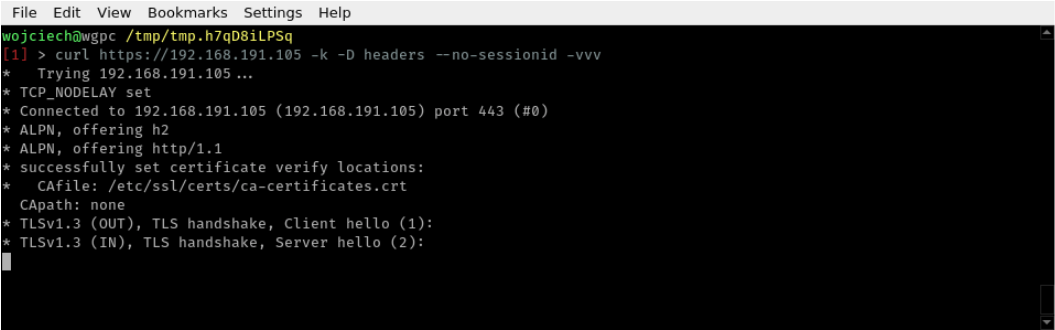
\includegraphics[width=\linewidth]{./images/2.png}

Usunięci flagi -k (zezwalajacej na nieznane certyfikaty) za drugim wykonaniem przyniosło ciekawszy efekt:

\begin{verbatim}
[130] > curl https://192.168.191.105 -D headers --no-sessionid -vvv
*   Trying 192.168.191.105...
* TCP_NODELAY set
* Connected to 192.168.191.105 (192.168.191.105) port 443 (#0)
* ALPN, offering h2
* ALPN, offering http/1.1
* successfully set certificate verify locations:
*   CAfile: /etc/ssl/certs/ca-certificates.crt
  CApath: none
* TLSv1.3 (OUT), TLS handshake, Client hello (1):
* TLSv1.3 (IN), TLS handshake, Server hello (2):
* TLSv1.2 (IN), TLS handshake, Certificate (11):
* TLSv1.2 (OUT), TLS alert, unknown CA (560):
* SSL certificate problem: self signed certificate in certificate chain
* Closing connection 0
curl: (60) SSL certificate problem: self signed certificate in certificate chain
More details here: https://curl.haxx.se/docs/sslcerts.html

curl failed to verify the legitimacy of the server and therefore could not
establish a secure connection to it. To learn more about this situation and
how to fix it, please visit the web page mentioned above.
\end{verbatim}

Logi serwera:
\begin{verbatim}
  . Performing the SSL/TLS handshake...
mbedtls_ssl_handshake line 6557

mbedtls_ssl_handshake line 6560
mbedtls_ssl_handshake line 6563 state 0
mbedtls_ssl_handshake line 6567 ret 0 state 1
mbedtls_ssl_handshake line 6563 state 1
mbedtls_ssl_handshake line 6567 ret 0 state 2
mbedtls_ssl_handshake line 6563 state 2
mbedtls_ssl_handshake line 6567 ret 0 state 3
mbedtls_ssl_handshake line 6563 state 3
mbedtls_ssl_handshake line 6567 ret 0 state 4
mbedtls_ssl_handshake line 6563 state 4
mbedtls_ssl_handshake line 6567 ret 0 state 5
mbedtls_ssl_handshake line 6563 state 5
mbedtls_ssl_handshake line 6567 ret 0 state 6
mbedtls_ssl_handshake line 6563 state 6
mbedtls_ssl_handshake line 6567 ret FFFFFFB0 state 7
mbedtls_ssl_handshake line 6573
mbedtls_ssl_handshake line 6576

 looping handshake
 failed
  ! mbedtls_ssl_handshake returned -80

Last error was: -80 - NET - Connection was reset by peer

  . Waiting for a remote connection …
\end{verbatim}

Teraz wariant z flagą -k też przechodzi do końca handshaku:
\begin{verbatim}
[60] > curl https://192.168.191.105 -D headers --no-sessionid -vvv -k
*   Trying 192.168.191.105...
* TCP_NODELAY set
* Connected to 192.168.191.105 (192.168.191.105) port 443 (#0)
* ALPN, offering h2
* ALPN, offering http/1.1
* successfully set certificate verify locations:
*   CAfile: /etc/ssl/certs/ca-certificates.crt
  CApath: none
* TLSv1.3 (OUT), TLS handshake, Client hello (1):
* TLSv1.3 (IN), TLS handshake, Server hello (2):
* TLSv1.2 (IN), TLS handshake, Certificate (11):
* TLSv1.2 (IN), TLS handshake, Server key exchange (12):
* TLSv1.2 (IN), TLS handshake, Server finished (14):
* TLSv1.2 (OUT), TLS handshake, Client key exchange (16):
* TLSv1.2 (OUT), TLS change cipher, Change cipher spec (1):
* TLSv1.2 (OUT), TLS handshake, Finished (20):
* TLSv1.2 (IN), TLS handshake, Finished (20):
* SSL connection using TLSv1.2 / ECDHE-RSA-AES256-GCM-SHA384
* ALPN, server did not agree to a protocol
* Server certificate:
*  subject: C=NL; O=PolarSSL; CN=localhost
*  start date: Feb 12 14:44:06 2011 GMT
*  expire date: Feb 12 14:44:06 2021 GMT
*  issuer: C=NL; O=PolarSSL; CN=PolarSSL Test CA
*  SSL certificate verify result: self signed certificate in certificate chain (19), continuing anyway.
> GET / HTTP/1.1
> Host: 192.168.191.105
> User-Agent: curl/7.63.0
> Accept: */*
\end{verbatim}



Między tymi kolejnymi wywołaniami projekt nie był rekompilowany, najwyżej resetowałem płytkę (a ostatnio sukcesy były bez resetu, jedynie przez goto).
Po resecie znów nie działa.

W niepoprawnej syuacji w wiresharku lecą tylko kolejne TCP Keep-Alive. NIe widać rozpoczęcia przesyłania cetyfikatu.

\subsection{2019-01-08}
Po pierwszy mflashowaniu po przyjściu do labu handshake przeszedł raz, potem
już nie.

Potem zmiana MACa ethernetif.c i tym samym nowe IP z DHCP (.102 zamiast .100).
Handshake przeszedł.
Potem restart płytki bez zmian i hadshake nie przeszedł.

Potem na routerze wymuszenie żeby ten nowy MAC dostał stare IP (.100).
Wymagało to restartu routera.

Teraz handshake przeszedł już 3 razy.


Zacząłem nagrywać wiresharkiem i wttejch wiliw nie przeszło. A już przechodziło
wielokrotnie po powrocie do oryginalnego MACa i IP.

Po zmianie MAC i dostani IP .102 (wireshark dale nagryw) przeszło kilka razy.

Wróciłem do defautlowego MACa (wireshark dalej nagrywa) - nie przechodzi.

\subsection{2019-01-13}

Powrót do PC. Po włączeniu i zresetowaniu płytka otrzymuje IP 192.168.191.105 (tak jak poprzednio, bo we wtorek zakończyłem chyba z oryginalnym MACiem. I znów nie przechodzi.
Wobec tego flashuję wersję ze zmionym MACiem, płytka dostaje IP 192.168.191.110 i działa.
Działa do pierwszego resetu, potem znów nie.
Po zmianie IP przez rezerwację DHCP (bez zmiany MAC) i resecie płytki nadal komunikacja zawiesza się na Server hello.

Sytuacja się powtarza:
zmiana adresu MAC w źródłach, flashowanie płytki
handshake wykonuje się poprawnie, również wielokrotnie (aż do resetu)
reset płytki
handshake zatrzymuje się na Server Hello

Po osiągnięciu stanu (4) nie działa również zapytanie z laptopa, sugerując że problem nie leży po stronie klienta.

Teraz nawet zmiana MACa (o parę wartości w jednym z pól) nie poamga. Zaczynam się zastanawiać, czy kluczem do problemu nie jest inicjalizacja wartości w jakimś nie-zawse-flashowanym obszarze pamięci.


Odłaczenie płytki od prądu i podłączenie również powoduje błędne zachowanie.
